\chapter{DB Partitioning as a RL Problem}
\label{db_partitioning}
\section{Reinforcement Learning}
Reinforcement learning is learning what to do - how to map situations to actions - so as to maximise a numerical reward signal. The learner is not told which actions yield the best rewards, but instead learns to discover which actions lead to the best rewards by trying them strategically. In the most challenging cases, such as learning how to find the best partitioning scheme in a database, actions such as choosing a partitioning scheme affect not only the immediate reward but also the next situation (where the agent needs to learn the next best partitioning scheme) and, through that, all subsequent rewards. These two characteristics - trial-and-error search and delayed reward- are the two most important distinguishing features of reinforcement learning \cite{sutton2018reinforcement}.

\citeauthor{sutton2018reinforcement} formalise the problem of reinforcement learning using ideas from dynamical systems theory, specifically, as the optimal control of incompletely-known Markov decision processes (MDPs). The basic ideas of MDPs capture the most important aspects of the real problem facing a learning agent interacting over time with its environment to achieve a goal. In the context of this thesis, the goal is to find the best partitioning scheme for a distributed database system. The agent must have a goal or goals relating to the state of the environment. MDPs consider three important aspects - sensation, action, and goal - in their simplest possible forms without trivialising any of them. 

It is also important to distinguish reinforcement learning from \textit{supervised learning} and \textit{unsupervised learning}. Supervised learning relies heavily on a training set of labelled examples provided by a knowledgeable external supervisor to learn a model that typically tries to solve a classification or a regression problem. On the other hand, unsupervised learning aims to usually find hidden patterns or structure hidden in collections of unlabelled data points. While reinforcement learning and unsupervised learning both deal with unlabelled data, it is important to distinguish them as reinforcement learning is trying to maximise a reward signal instead of trying to find a hidden structure \cite{sutton2018reinforcement}. Since our learning agent does not rely on learning the best partitioning schemes from historical labelled cost execution costs of different query workloads on a distributed DBMS, our problem is not a supervised learning problem. Neither is it trying to find hidden patterns in any past historical data - hence, it is not an unsupervised learning problem.

\section{Markov Decision Processes}

MDPs are a classical formalisation of sequential decision making, where actions influence not just immediate rewards, but also subsequent situations or states, and through those future rewards \cite{sutton2018reinforcement}. In MDPs, we estimate the value $q_*(s,a)$ of each action $a$ in each state $s$ or the value $v_*(s)$ of each state given optimal action selections. MDPs effectively frame the problem of learning from interaction to achieve a goal. The learner and decision maker is called the \textit{agent}. The thing it interacts with, comprising everything outside the agent, is called the \textit{environment}. The environment and the agent interact continually - the agent selects the actions and the environment responds to those actions and presents new \textit{states} to the agent. The environment creates \textit{rewards} - special numeric values that the agent seeks to maximise over time through its choice of actions \cite{sutton2018reinforcement}. 

The agent and environment interact in discrete time steps, $t = 0,1,2,3, ...$. At each time step $t$, the agent receives a representation of the environment's \textit{state}, $s_t$ and on that basis selects an \textit{action}, $a_t \in A$. After every time step, the agent receives a numerical \textit{reward}, $r_t$ based on a consequence of its action, and finds itself in a new state $s_{t+1}$. 

% Insert picture here
\begin{figure}[h]
  \centering
  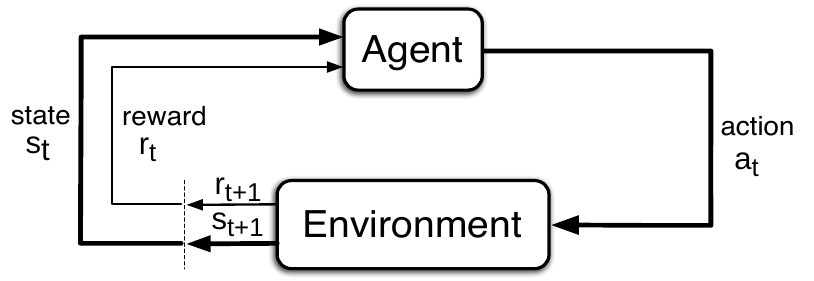
\includegraphics[width=\linewidth]{figures/mdp_ag_env_interaction.png}
  \caption{The agent environment interaction in a Markov Decision Process.}
%   \Description{The agent environment interaction in a Markov Decision Process.}
\end{figure}


\section{Policies and Value Functions}
All reinforcement learning algorithms rely on \textit{value functions} in order to estimate \textit{how good} it is for the agent to be in a given state. The idea of "how good" a state is is defined in terms of expected returns. Rewards, however, are dependent upon the actions that the agent will take and as such, value functions are defined with respect to particular ways of acting, called \textit{policies}. 
Formally, a \textit{policy} is a mapping from states to probabilities of selecting each possible action \cite{sutton2018reinforcement}. If an agent is following policy $\pi$ at time $t$, then $\pi(a|s)$ is the probability that $a_t=a$ if $s_t=s$. An example of a policy is a greedy policy, which involves selecting the action with the highest immediate reward. However, a greedy policy might not always be the best strategy and instead, the agent might seek to select an action that enables higher rewards in the future while keeping long-term higher rewards in mind. 
In terms of database partitioning, \citeauthor{Hilprecht:2019:TLP:3329859.3329876} opted to solve the problem using \textit{Q-learning} \cite{Hilprecht:2019:TLP:3329859.3329876, DBLP:conf/sigmod/HilprechtBR20}.   

\section{Deep Q-Learning}
\label{sec:q-learning}
Q-Learning was considered one of early breakthroughs in reinforcement learning since it is considered an off-policy control algorithm \cite{watkins1992q}.
\begin{equation}
\label{eq:bellman}
Q(s_t,a_t) \xleftarrow[]{} Q(s_t,a_t) + \alpha[r_{t+1} + \gamma \max_a Q(s_{t+1},a) - Q(s_t,a_t)]
\end{equation}
The learned action-value function, $Q$, directly approximates $q_*$, the optimal action-value function, independent of the policy being followed \cite{sutton2018reinforcement}. Q-learning is considered off-policy because it learns from actions that are outside the current policy, e.g. taking random actions. Specifically, q-learning seeks to learn a policy that maximises the total reward. 
With the Q-function, the expected discounted future rewards are approximated as follows, if we pick action $a$ at state $s$:
\begin{equation}
    Q(s,a) = \mathbb{E}\bigg(\sum^{\infty}_{t=0}r_t(s_t,a_t)\gamma^t|s_0=s,a_0=a \bigg)
\end{equation}
The rewards are discounted with a factor $\gamma < 1$ to account for a higher degree of uncertainty for later states. If the approximation is good enough we can choose an optimal action for a state $s$ as $\text{argmax}_{a \in A} Q(s,a)$. Selecting random actions offers a trade-off between exploration and exploitation during training the advisor. Usually, exploration is performed by picking a random action with probability $\epsilon$. This probability is decayed over time \cite{sutton2018reinforcement} by multiplication with a factor called \textit{epsilon decay}. 

The optimal action-value function obeys an important identity known as the \textit{Bellman equation}. This is based on the following intuition: if the optimal value $Q^*(s',a')$ off the sequence $s'$ at the next time-step was known for all possible actions $a'$, then the optimal strategy is to select the action $a'$ minimising the expected value of $r + \gamma Q^*(s',a')$.
The basic idea behind many reinforcement learning algorithms is to estimate the action-value function, by using the Bellman equation as an iterative update, $Q_{i+1}(s,a) = \mathbb{E}[r+\gamma \max_{a'}Q_i(s',a')| s,a]$. Such \textit{value iteration} algorithms converge to the optimal action-value function, $Q_i \xrightarrow[]{} Q^*$ as $i \xrightarrow[]{} \infty$\cite{sutton2018reinforcement}. In practical, this approach is impractical, because the action-value function is estimated separately for each sequence, without any generalisation. 

One of the ways of realising the Q-function is through Deep-Q-Learning (or Deep Reinforcement Learning) \cite{Zhu:2017:BTP:3127479.3128605}.  For Deep-Q-Learning, a neural network $Q_\theta(s,a)$ with weights $\theta$ is used for the approximation. Having observed a state $s_t$ and an action $a_t$, the corresponding immediate reward $r_t$ and the future state $s_{t+1}$ the network is updated via Stochastic Gradient (SGD) and the squared error loss:
\begin{equation}
    \bigg( r_t + \gamma\ \max_{a \in A} Q_\theta(s_{t+1},a_t) - Q_\theta(s_t, a_t) \bigg)^2
\end{equation}
The intuition is that the expected discounted future rewards when selecting action $a_t$ in step $t$ should be the immediate reward $r_t$ plus the maximum expected discounted future rewards when selecting the best action $a$ in the next step $t+1$ discounted by $\gamma$, i.e. $\text{argmax}_{a \in A} Q(s_{t+1},a)$. This process can be summarised as shown in Figure~\ref{fig:dqn}, which shows the closed loop Deep-Q-Learning approach.

\begin{figure}[h]
  \centering
  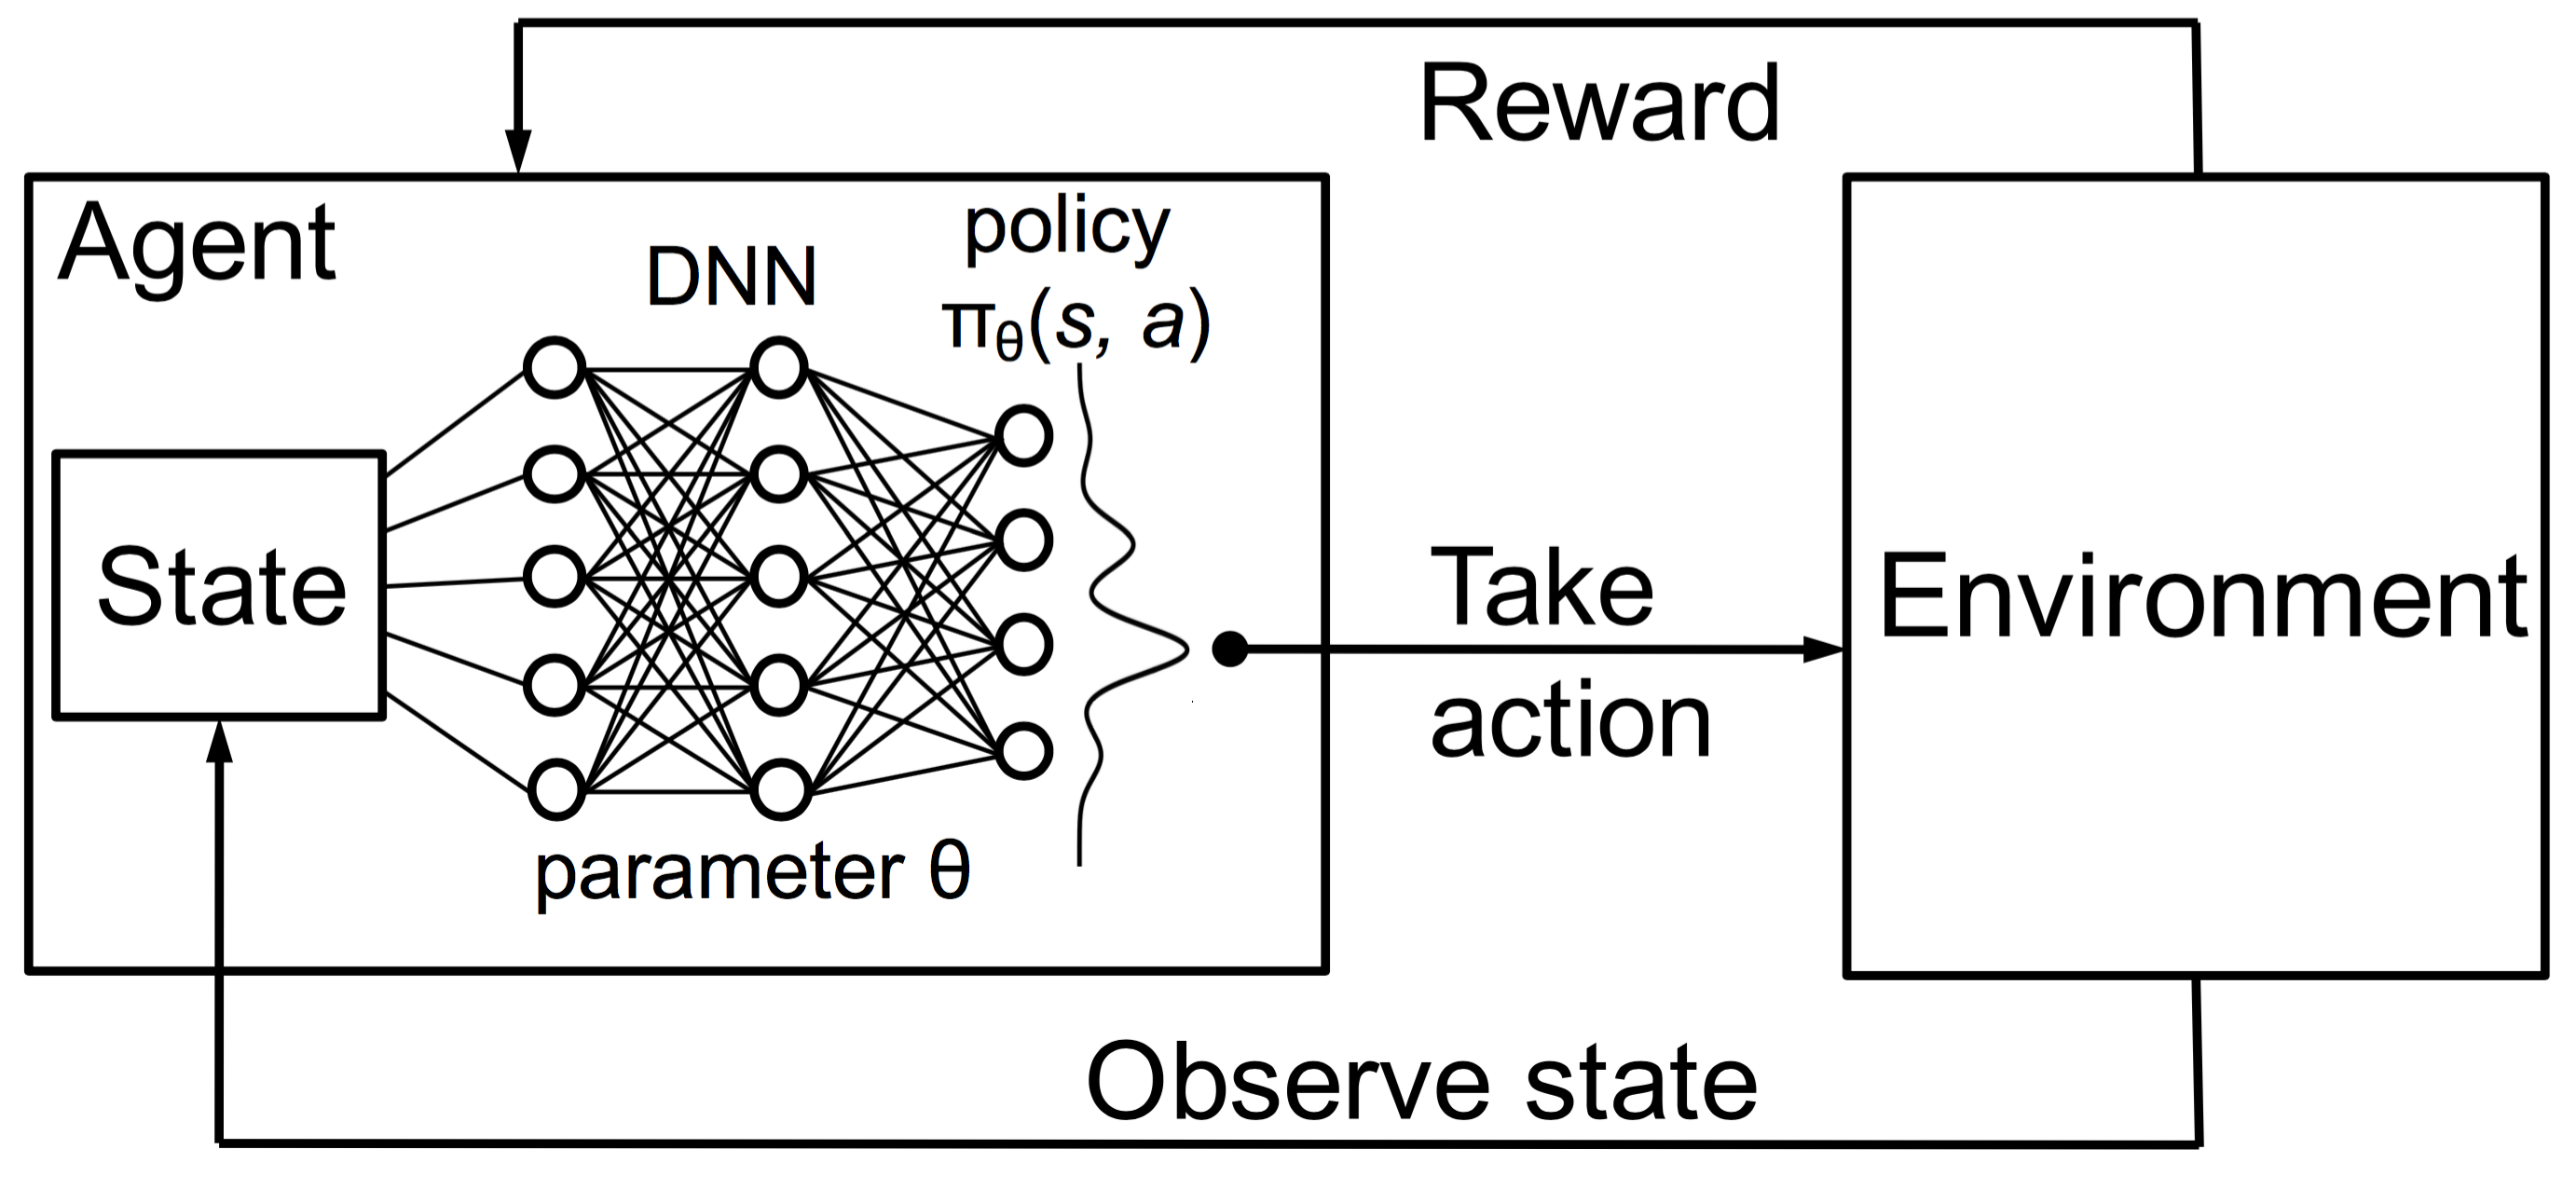
\includegraphics[width=\linewidth]{figures/dqn.png}
  \caption{Closed loop Deep-Q Reinforcement Learning}
%   \Description{The agent environment interaction in a Markov Decision Process.}
  \label{fig:dqn}
\end{figure}


\section{Problem Formulation}
Using DRL to find an optimal partitioning scheme is a relatively novel idea \cite{Hilprecht:2019:TLP:3329859.3329876, DBLP:conf/sigmod/DurandPPMBSSRB18}. \citeauthor{Hilprecht:2019:TLP:3329859.3329876} formally described a partitioning problem as follows: Given a set of tables $T$ and queries $Q$, for every table $T_i \in T$ with attributes $a_{i1}, a_{i2}, ...a_{in}$, the agent has to decide whether to replicate or to partition the table. For simplicity, only one partitioning scheme (e.g., hash-partitioning) that horizontally splits a table into a fixed number of shards (equal to the number of nodes in the database cluster) is considered. This provides the benefit of locality of data on the same node if two tables are co-partitioned on a attribute, and as such, equi-joins do not require any data shuffling. For replication, if a table is selected to be replicated, it is replicated across all nodes. In summary, there are two problems: i) selecting whether to replicate or partition a table and ii) for the latter, which attribute $a_i$ (or set of attributes) to partition on. 

The main intuition to model the partitioning as a DRL problem is as follows:
\begin{itemize}
    \item model the database and the workload as \textit{state}
    \item model the possible changes in the partitioning scheme as \textit{actions}
    \item model the actual runtime (online phase) or the estimated runtime (offline phase) of the cost model as \textit{rewards}
\end{itemize}

For training a partitioning advisor, the DRL agent interacts with the state reflecting the current partitioning by selecting different actions and observing rewards as described earlier. The actions in the model change the current partitioning and the rewards to represent the total cost to run a given mix of queries \cite{Hilprecht:2019:TLP:3329859.3329876, DBLP:conf/sigmod/HilprechtBR20}. 
As an optimisation technique, \citeauthor{Hilprecht:2019:TLP:3329859.3329876} perform the training in two phases an i) \textbf{offline phase} and an ii) \textbf{online phase.} In the offline phase, the runtimes of different partitioning $P$ are only approximated with a cost model $c_m(P,q_i)$. This provides the benefit of not having to run actual queries on the database, thus speeding up the initial training process. The online phase then takes over from where the offline phase leaves the model and proceeds to train the model on actual runtimes - thus refining the model learnt from the offline phase. The complete approach is covered in Section~\ref{Methods} of this thesis.

